\section{Παρουσίαση αποτελεσμάτων}

\subsection{Προφίλ ταχύτητας στην αξονική θέση του δρομέα}

\begin{figure}[h!]
    \begin{center}
        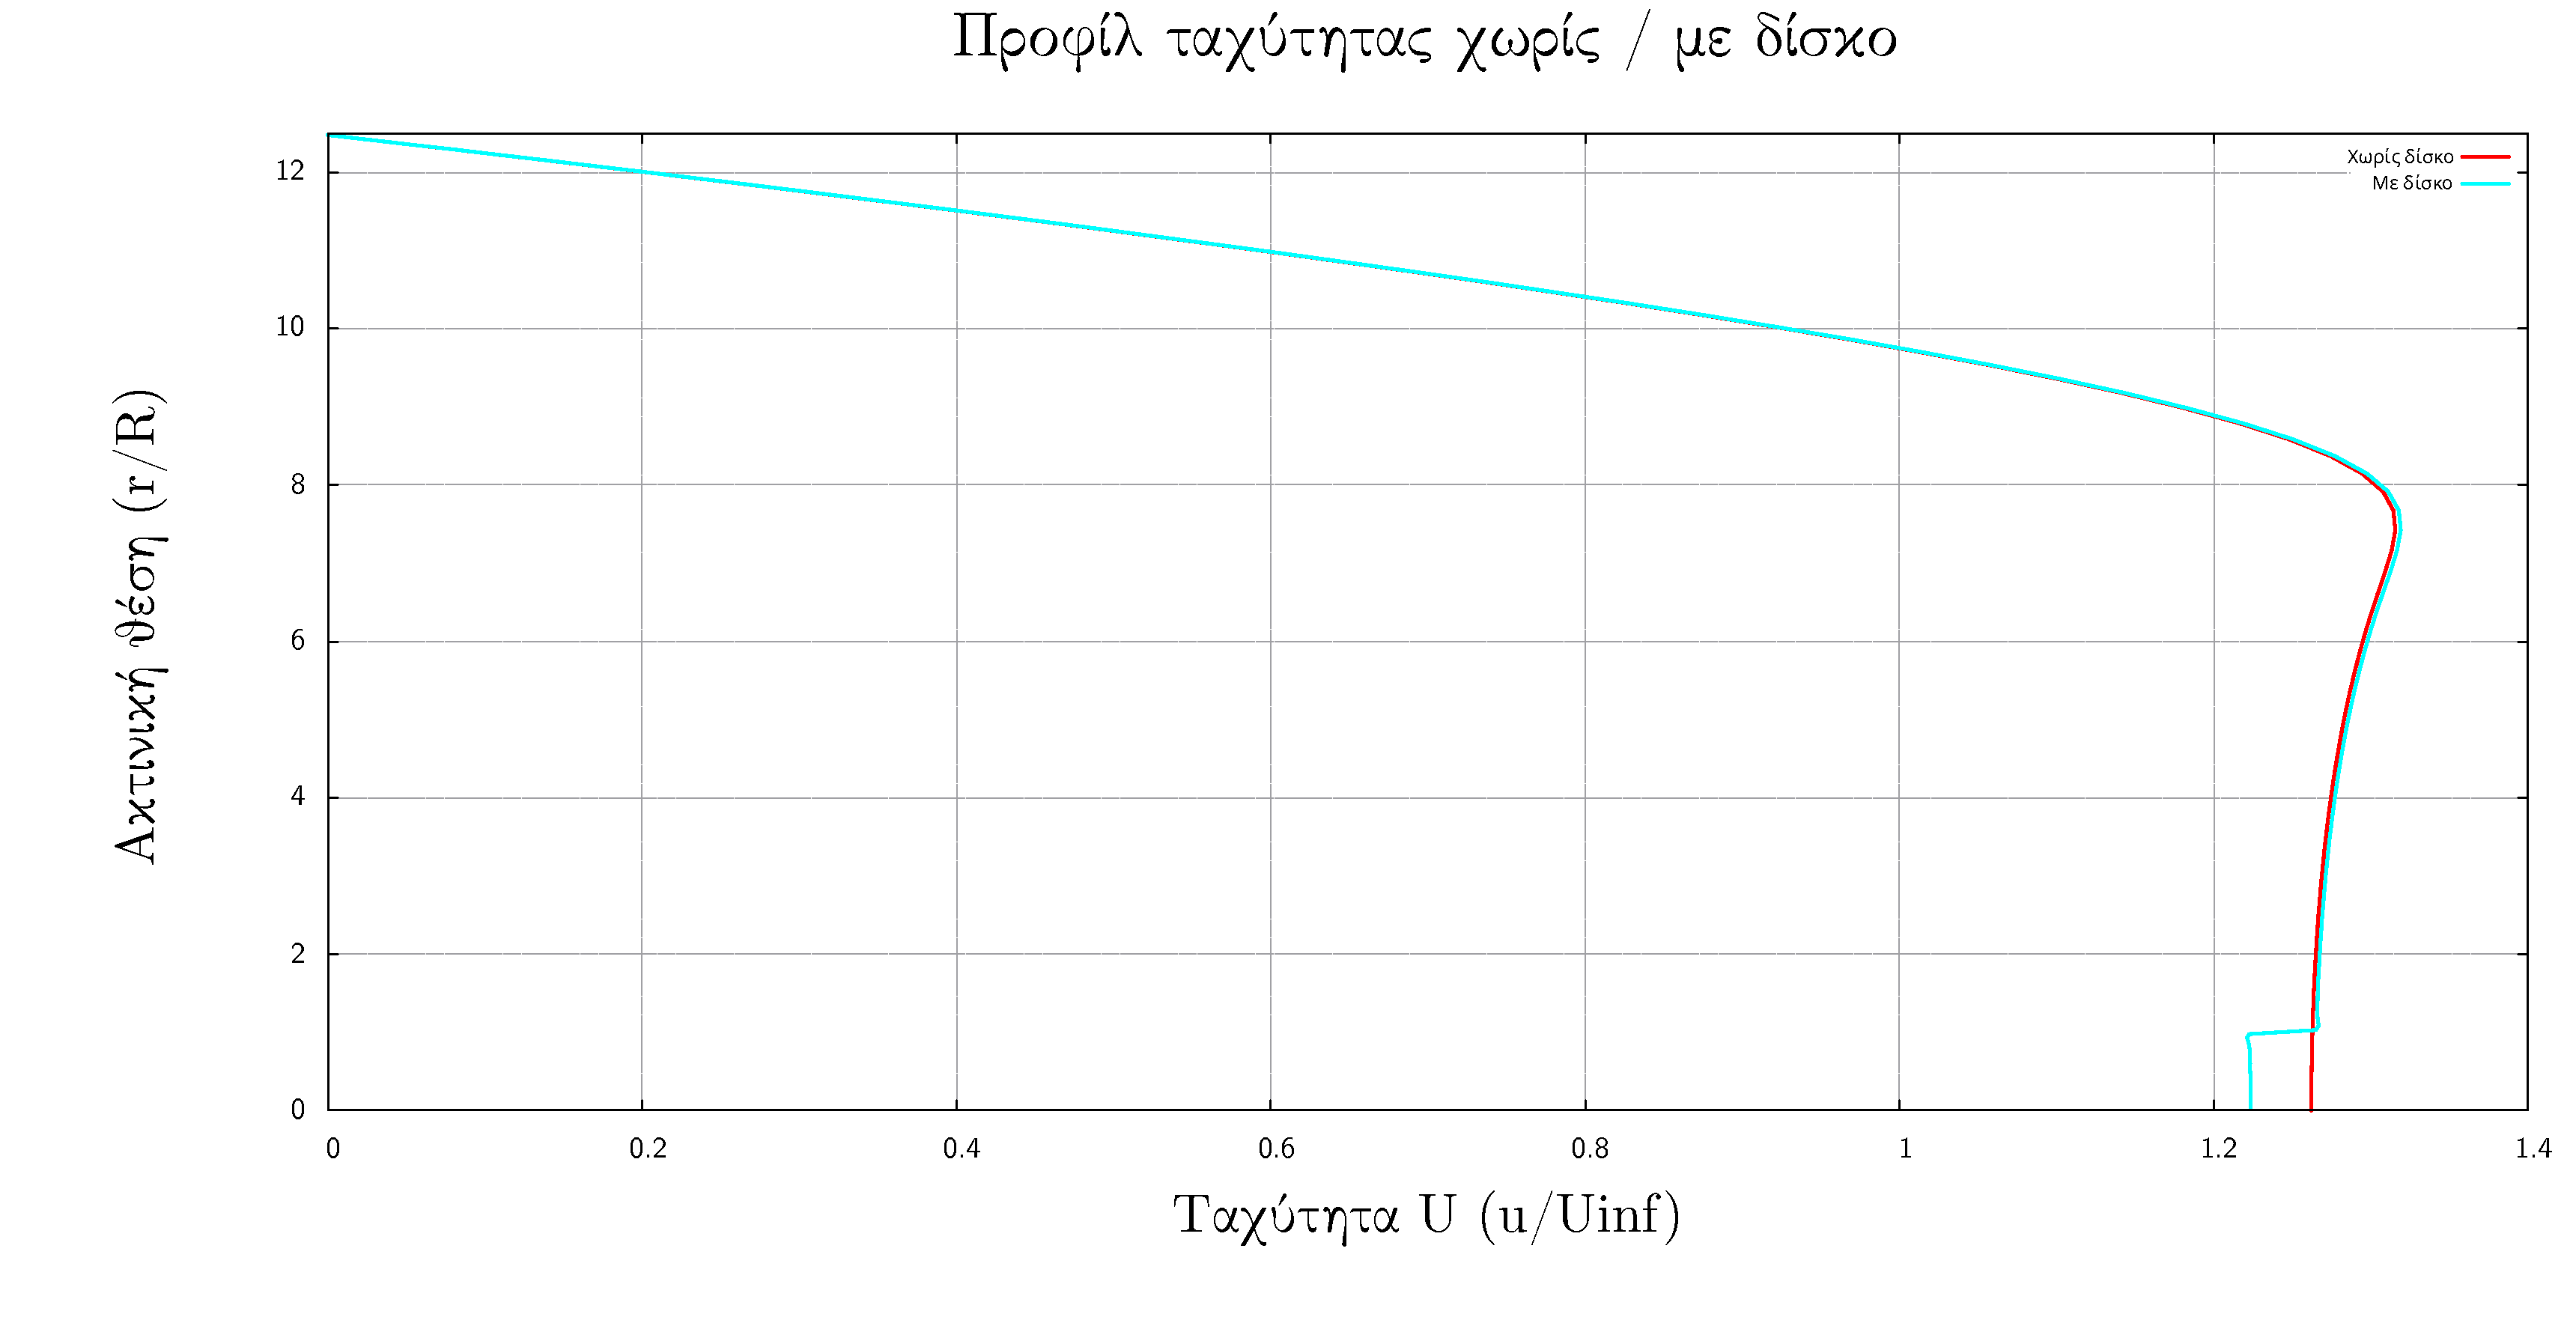
\includegraphics[width=0.75\textwidth]{figures/x0_prof.pdf}
    \end{center}
    \caption{Αξονική θέση του δρομέα}
    \label{fig:x0prof}
\end{figure}

\newpage
\subsection{Ισοταχείς της ροής παρουσία δρομέα}

\begin{figure}[h!]
    \begin{center}
        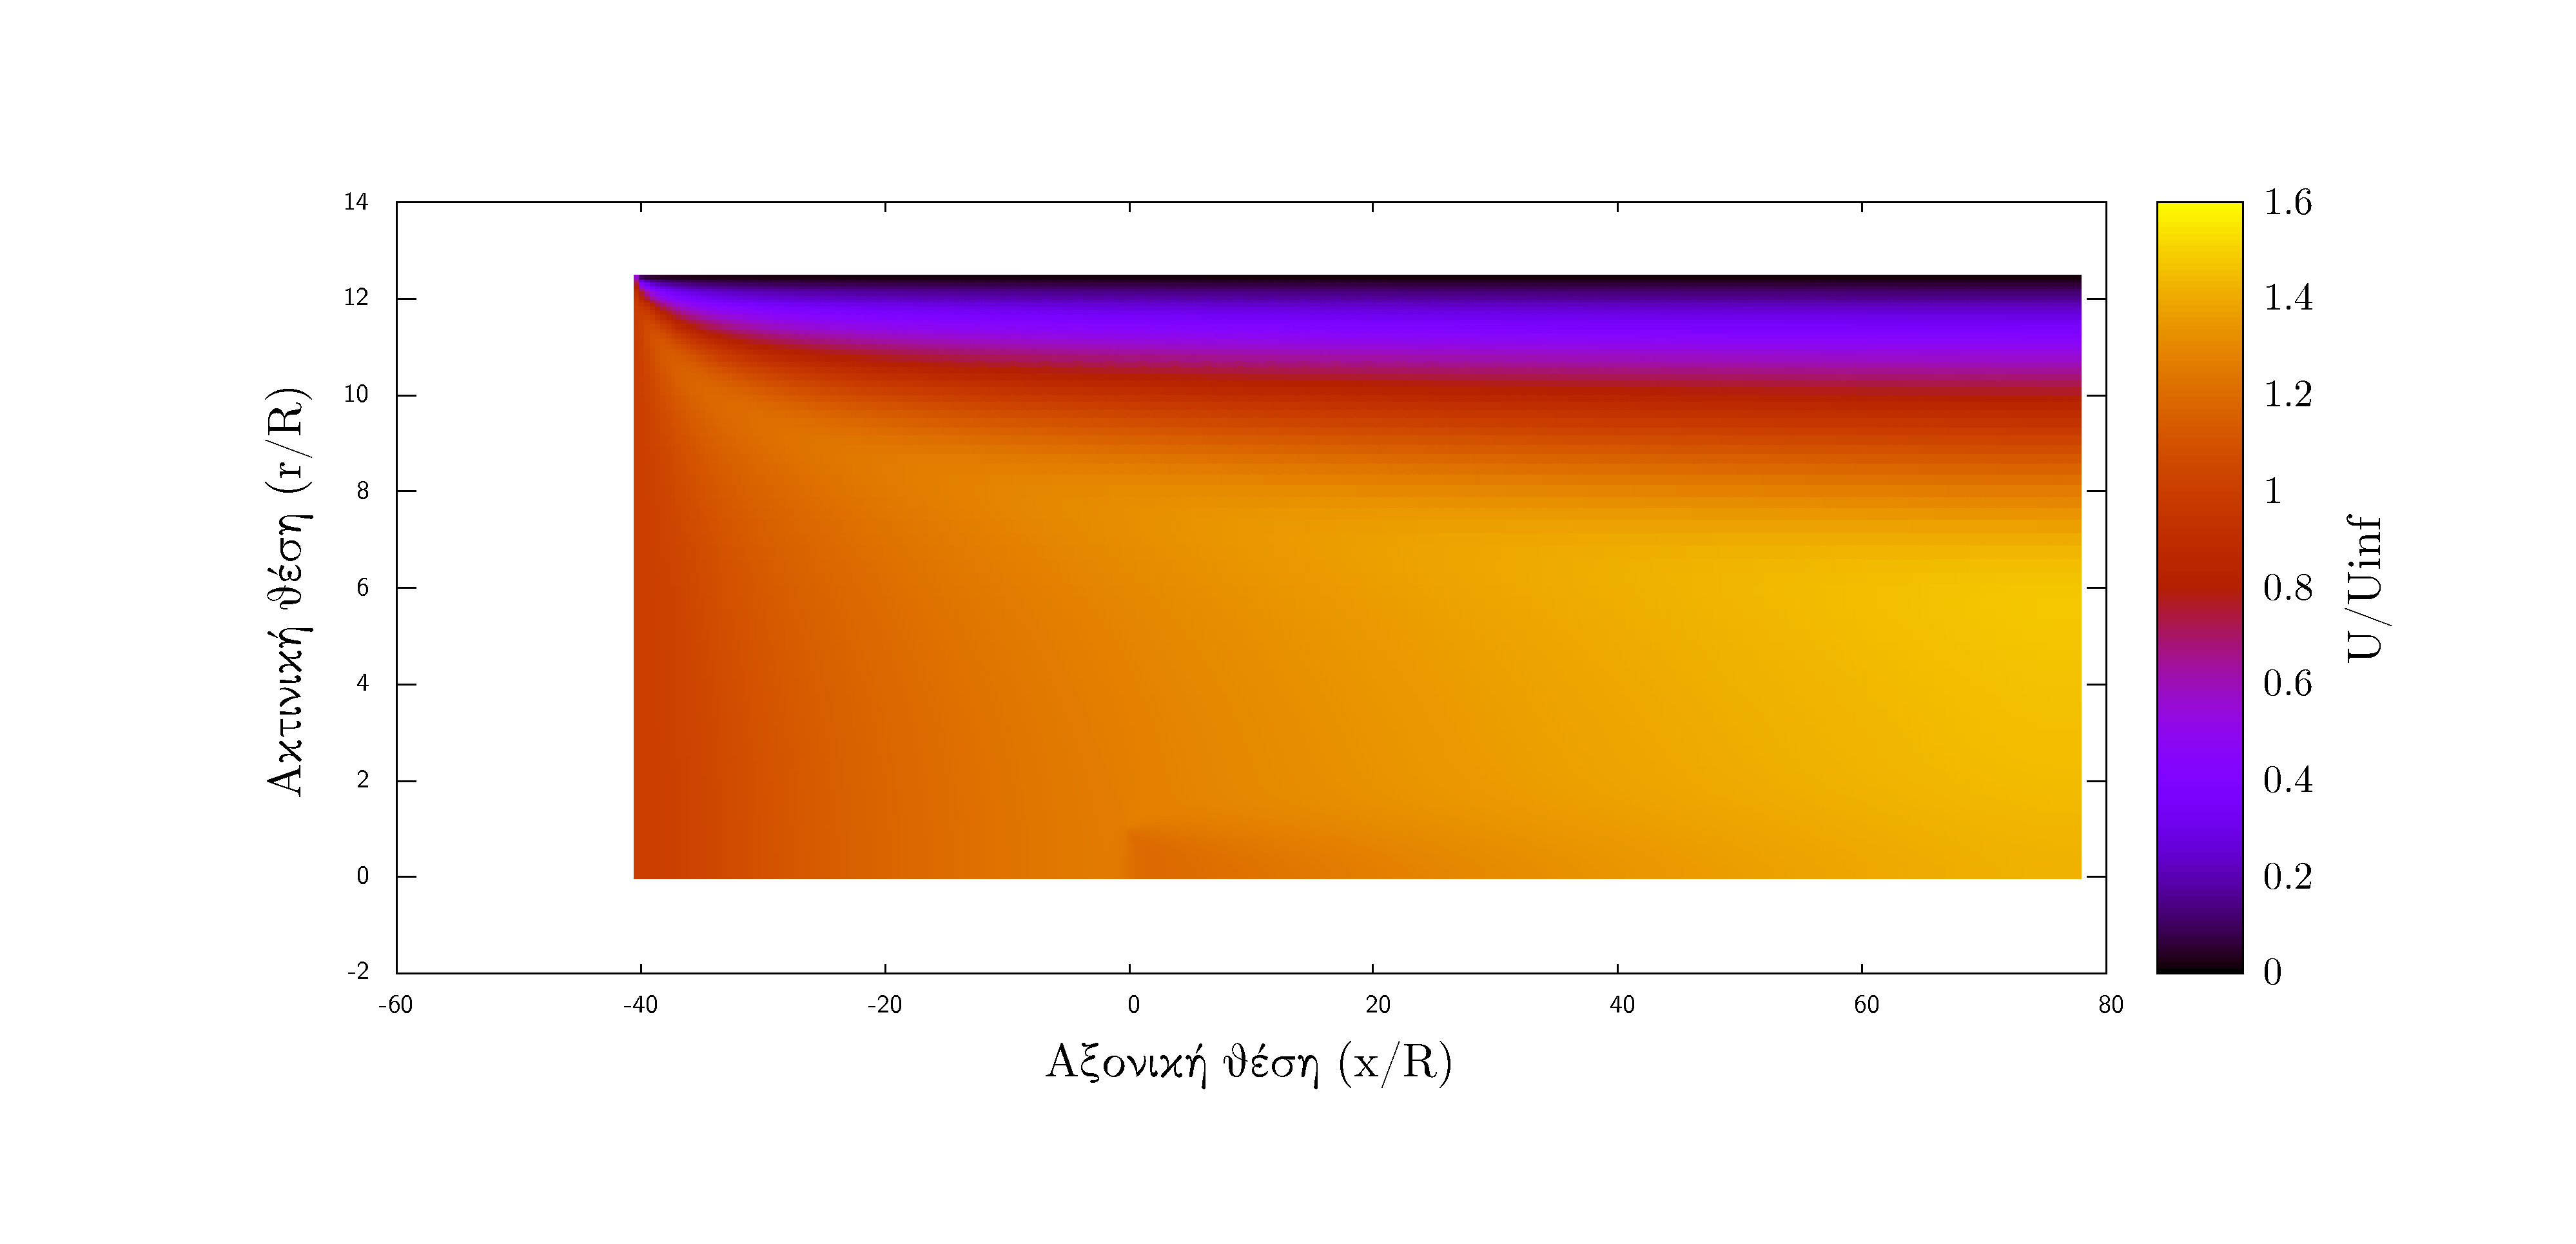
\includegraphics[width=0.85\textwidth]{figures/isoU.pdf}
    \end{center}
    \caption{Ισοταχείς του πεδίου ροής}
    \label{fig:isoU}
\end{figure}

\begin{figure}[h!]
    \begin{center}
        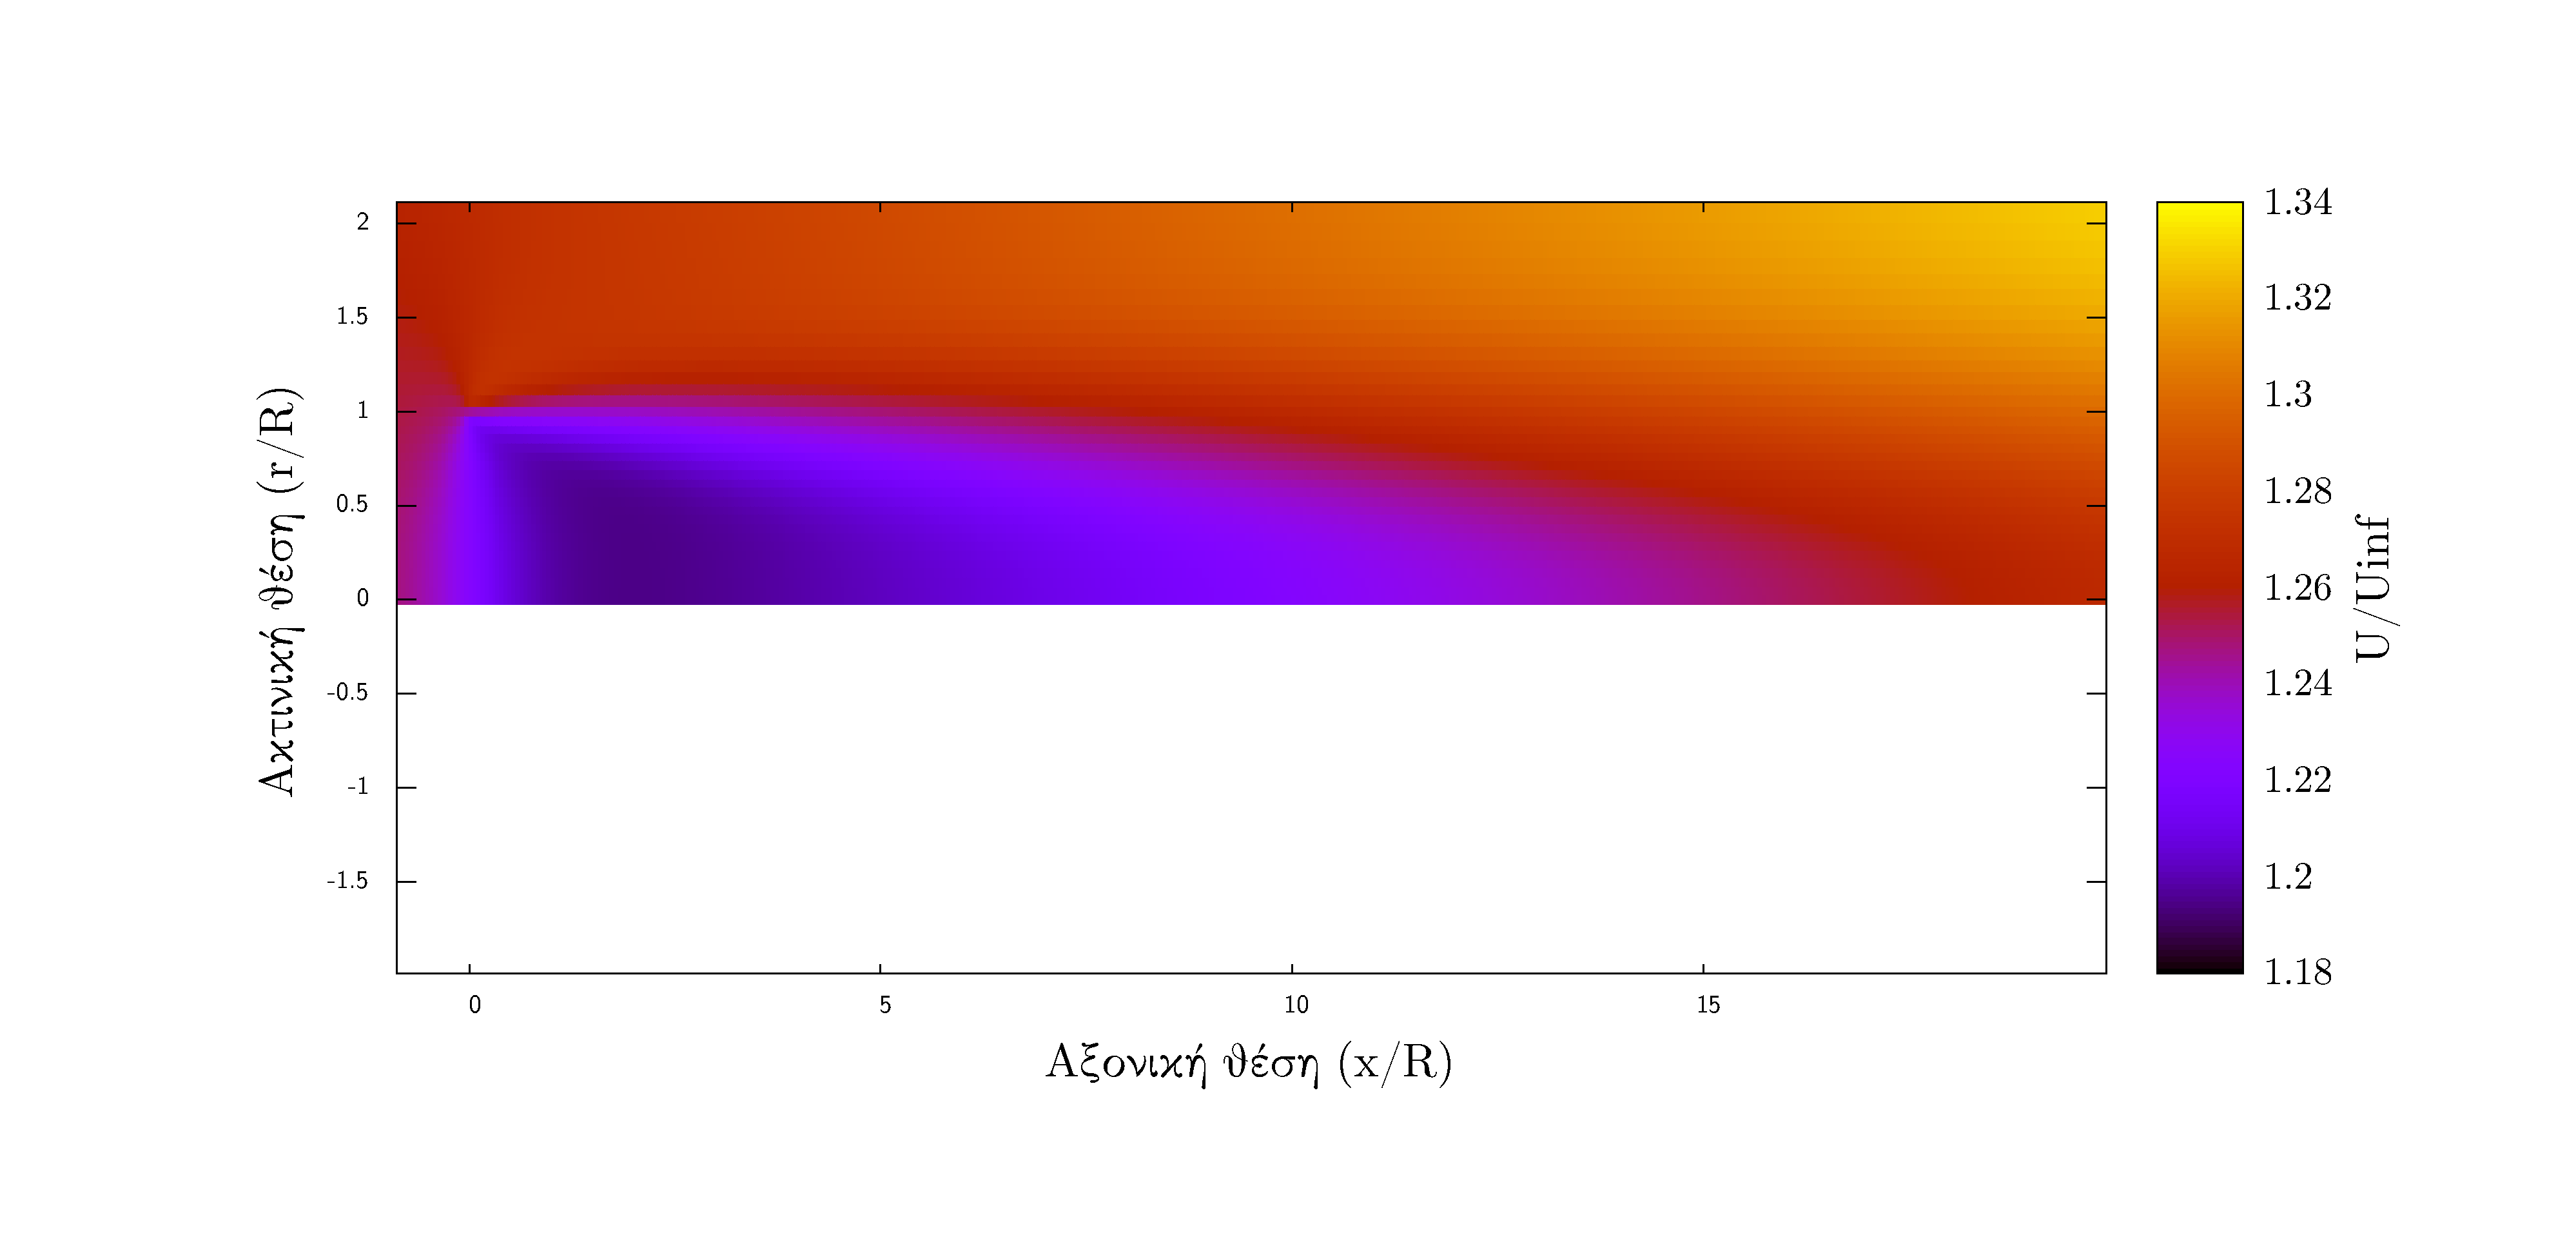
\includegraphics[width=0.85\textwidth]{figures/isoU_zoom.pdf}
    \end{center}
    \caption{Ισοταχείς του πεδίου ροής - μεγέθυνση στην περιοχή του δρομέα}
    \label{fig:isoU_zoom}
\end{figure}

\subsection{Προφίλ μεγεθών κατάντι του δρομέα}

\begin{figure}[h!]
    \begin{center}
        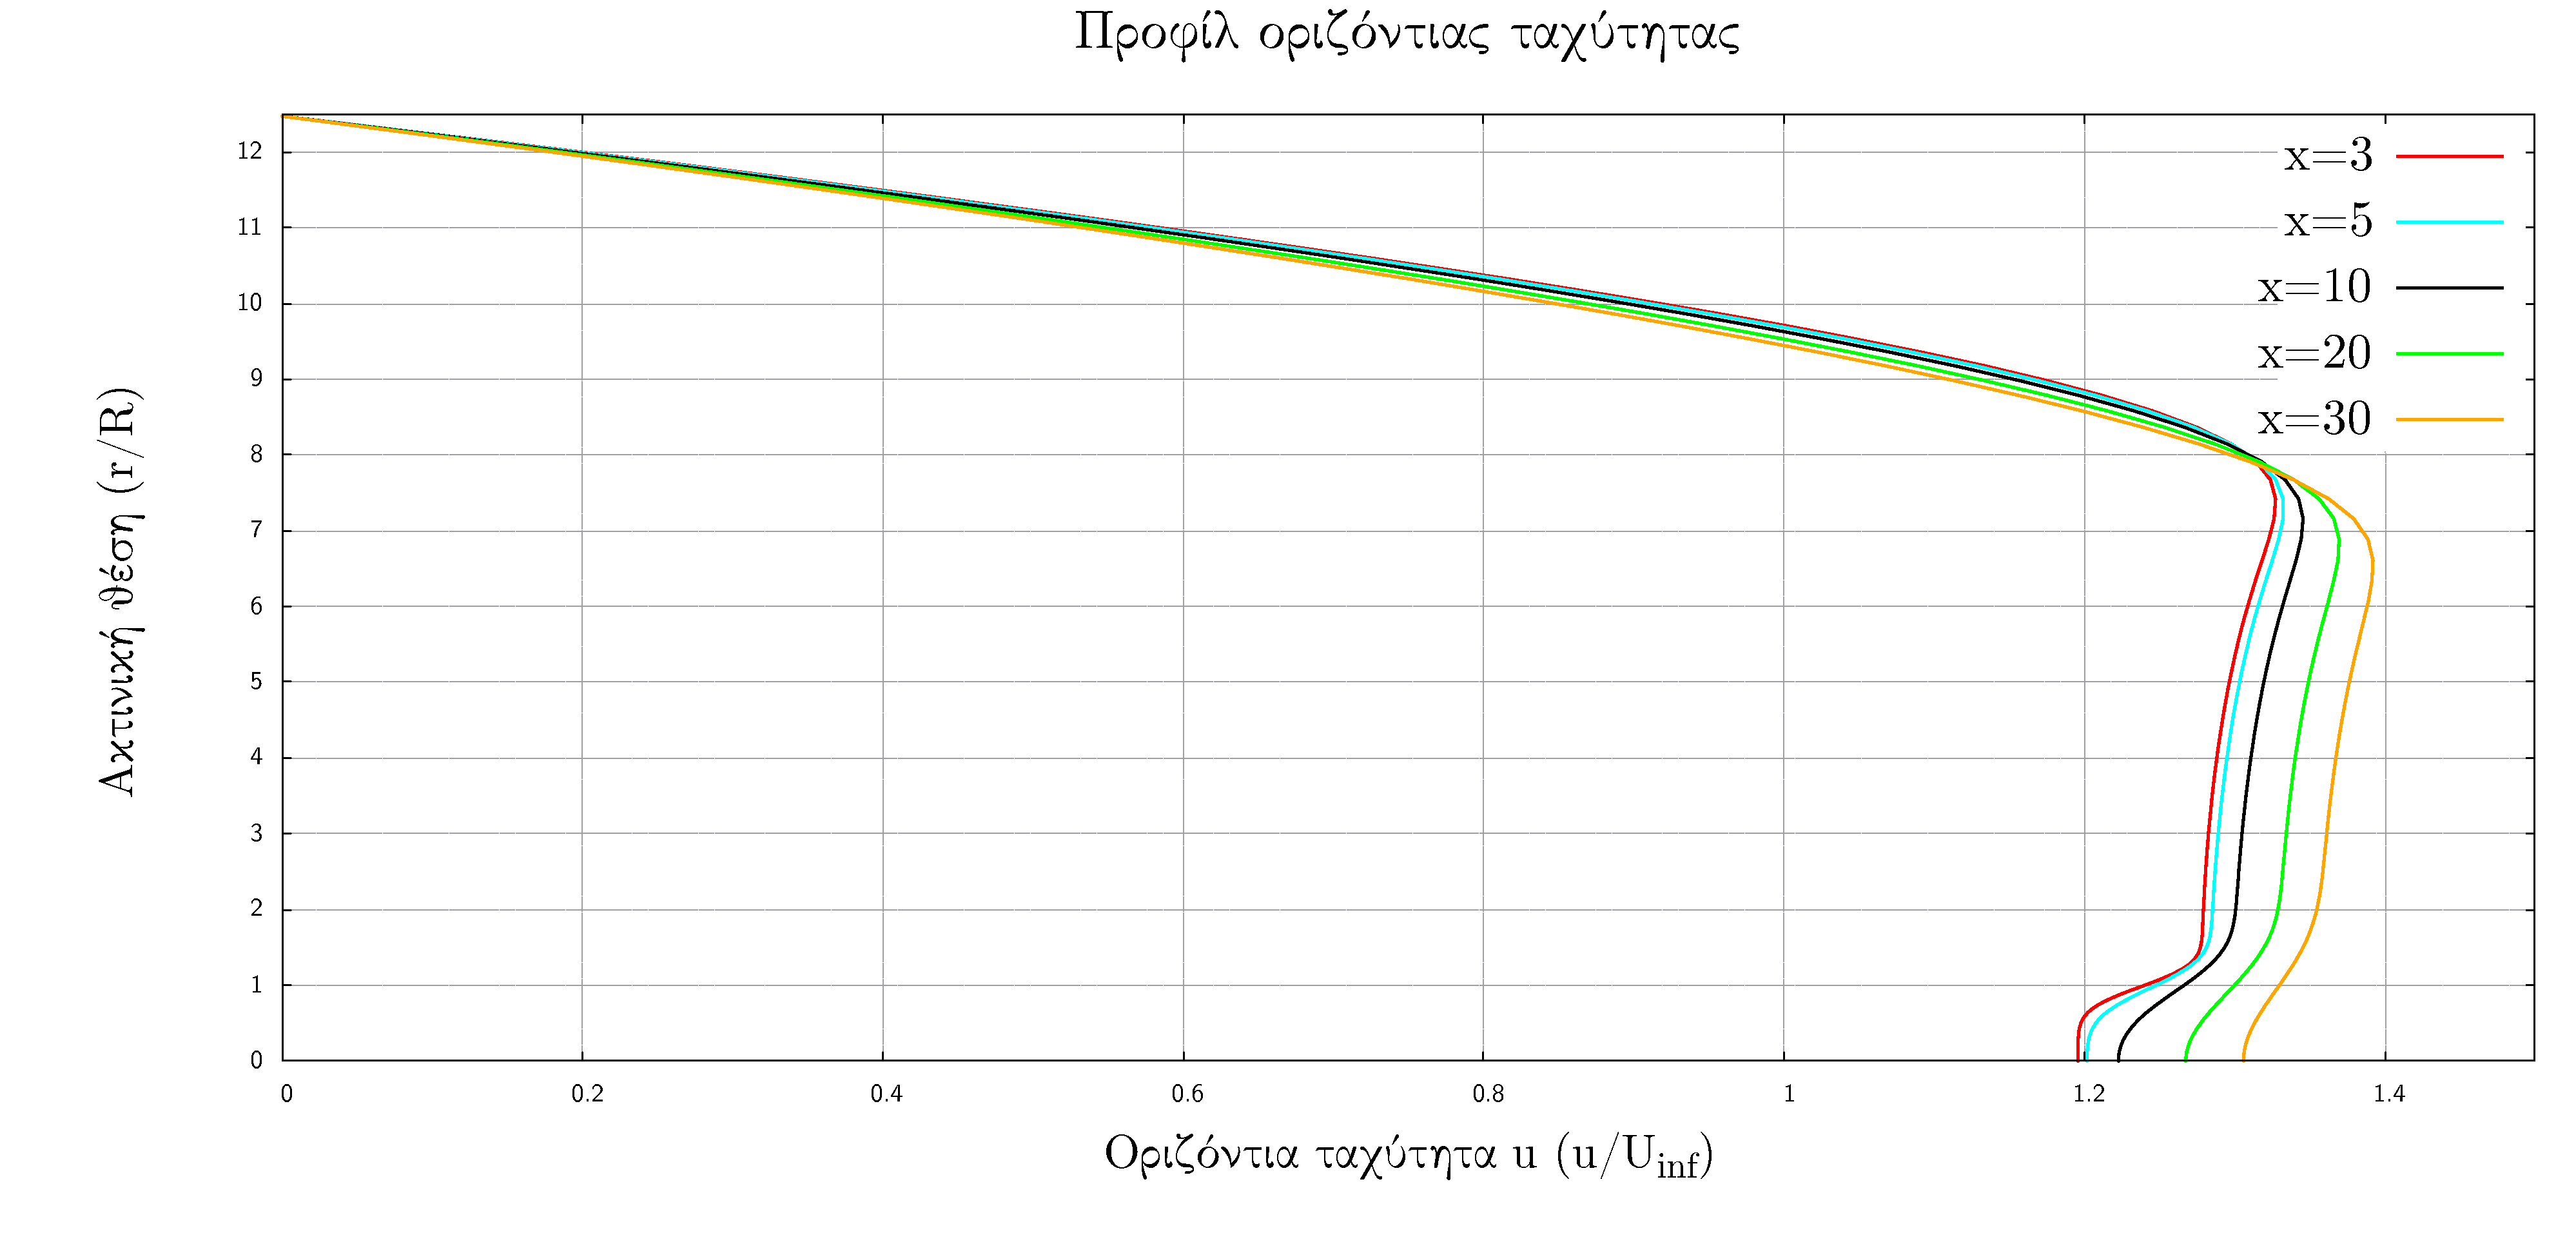
\includegraphics[width=0.85\textwidth]{figures/u_B.pdf}
    \end{center}
\end{figure}

\begin{figure}[h!]
    \begin{center}
        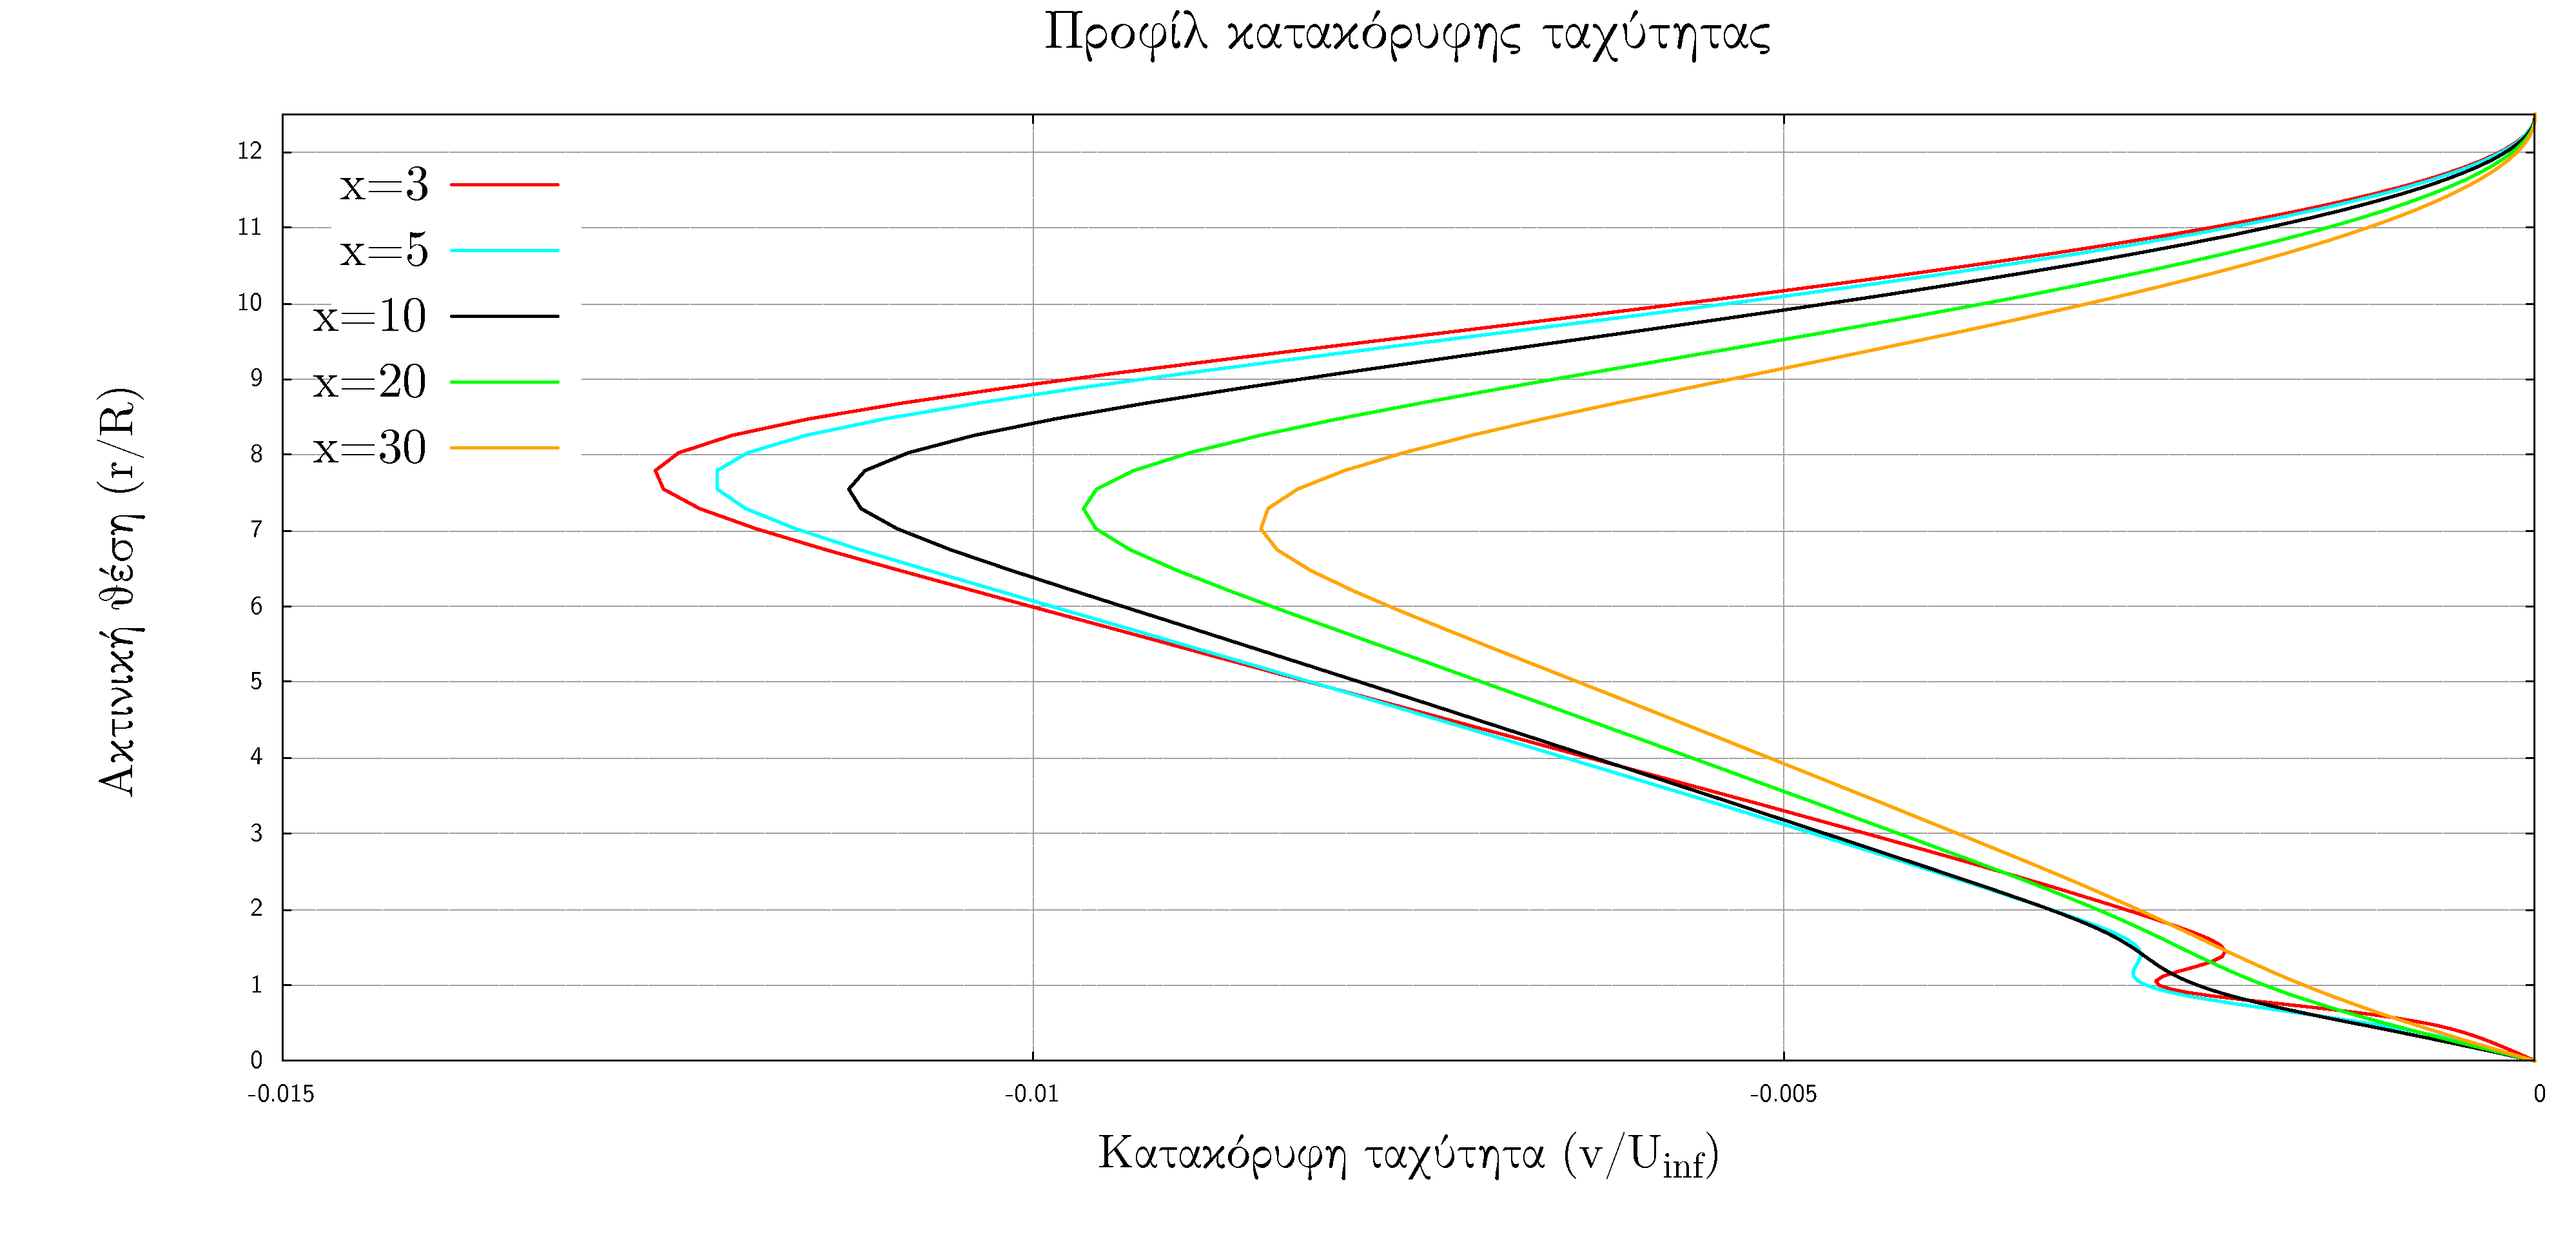
\includegraphics[width=0.85\textwidth]{figures/v_B.pdf}
    \end{center}
\end{figure}

\begin{figure}[h!]
    \begin{center}
        \includegraphics[width=0.85\textwidth]{figures/TE_B.pdf}
    \end{center}
\end{figure}
